\documentclass[11pt]{article}
\usepackage[hmargin=1in,vmargin=1in]{geometry}
\usepackage{xcolor}
\usepackage{amsmath,amssymb,amsfonts,url,sectsty,framed,tcolorbox,framed}
\usepackage{multicol}
\setlength{\columnsep}{0.5cm}
\usepackage{blindtext}
\usepackage{tikz}
\usepackage{graphicx}

\newcommand{\pf}{{\bf Proof: }}
\newtheorem{theorem}{Theorem}
\newtheorem{lemma}{Lemma}
\newtheorem{proposition}{Proposition}
\newtheorem{definition}{Definition}
\newtheorem{remark}{Remark}
\newtheorem{th}{}

\newcommand{\qed}{\hfill \rule{2mm}{2mm}}


\begin{document}
%%%%%%%%%%%%%%%%%%%%%%%%%%%%%%%%%%%%%%%%%%%%%%%%%%%%%%%%%%%%%%%%%%%%%

\noindent
\rule{\textwidth}{1pt}
\begin{center}
{\bf [CS304] Introduction to Cryptography and Network Security}
\end{center}
Course Instructor: Dr. Dibyendu Roy \hfill Winter 2022-2023\\
Scribed by: Rathva Kaushikkumar Sanjaybhai (202051156) \hfill Week : 2 (4nd lecture \#)
\\
\rule{\textwidth}{1pt}

%%%%%%%%%%%%%%%%%%%%%%%%%%%%%%%%%%%%%%%%%%%%%%%%%%%%%%%%%%%
%write here

\section{Kirchhoff's Rule :}
Design of cryptographic algorithm needs to be public in order of it to be :
\begin{enumerate}
    \item Widely adapted by people.
    \item For the algorithm to improve.
\end{enumerate}

\section{The perfect Secrecy : Shonno's notion}
Encryption algo \quad E\\ 
Message \quad M \\
Cipher text \quad C \\\\
E(M) = C\\
 Here C might transmitted through public domain where people read it.
\begin{definition}
\textbf{\underline{Perfect Secrecy}} : E will be providing perfect secrecy if the cipher text doesn't reveal any information regarding the plain text/message.\\
When we have the cipher text.

For the perfect secrecy the reader shouldn't have any advantage over the situation where they doesn't have it.
\end{definition}\\

$P_r[M=m | C=c]=P_r[M=m]\\

P_r[message | Cipher text] = P_r[message]$\\

If probability of us guessing the answer right \underline{without cipher text is $p_g$} and \underline{with cipher text is $p_c = p_g+\epsilon$}.
\begin{th}
Then $p_c$ should be less or equal to $p_g$.\\
So,
$p_c\ \le \ p_g\\
p_g+\epsilon \le p_g $
\end{th}

 \footnote{OTP - One Time Padding.}
\newpage


\section{Symmetric Key Cipher :}
\textbf{Symmetric Key Cipher has two categories :}

\subsection{Block cipher :}
\underline{M message} is devided in \underline{n blocks} of fixed \underline{length l}.\\

$M\ =\ m_0\ ||\ m_1\ ||\ m_2\ ||\ .\ .\ .\ ||\ m_n$ $\rightarrow$ Blocks

\subsubsection[*]{Encryption :}
Enc is encryption function.\\

$C\ =\ Enc(m_0,k)\ ||\ Enc(m_1,k)\ ||\ .\ .\ .\ Enc(m_n,k)$\\

$C\ =\ (c_0\ ||\ c_1\ ||\ c_2\ .\ .\ .\ ||\ c_n)$\\

\subsubsection[*]{Decryption :}
Dec is encryption function.\\

$C\ =\ Dec(c_0,k)\ ||\ Dec(c_1,k)\ ||\ .\ .\ .\ Dec(c_n,k)$\\

$Plain\ text\ =\ (p_0\ ||\ p_1\ ||\ p_2\ .\ .\ .\ ||\ p_n)$\\

Block cipher is not very efficient for long strings.
\subsection{Stream Cipher :}
Stream cipher is used in places where the length of the message to be encrypted is either too long or length is not determined just yet.\\

For example, Mobile telephony and easy hardware implementation.\\

$M\ =\ (m_0\ .\ .\ .\ m_n)$ where $m_n\ \epsilon \ {0,1}$
\subsubsection[*]{Encryption :}

$C\ =\ (m_0 \oplus z_0 ,m_1 \oplus z_1\ .\ .\ .\ m_n \oplus z_n) $\\

Here, $z_0,z_1 .\ .\ .\ z_n$ are generated using function $F(k)\ \rightarrow z_i \epsilon {0,1}$

\subsubsection[*]{Decryption :}

$Plain text \ =\ (c_0 \oplus z_0 ,c_1 \oplus c_1\ .\ .\ .\ c_n \oplus z_n) $\\

\newpage

\section{Product Cipher :}
A product cipher \textbf{combines two or more transformations} in a manner intending that the \textbf{resulting cipher is more secure} then the individual transformations.

\section{Substitution Permutation Network (SPN):}
It is a product cipher based substitution box and permutation box,
SPN is based on block cipher and AES is based on SPN.\\\\
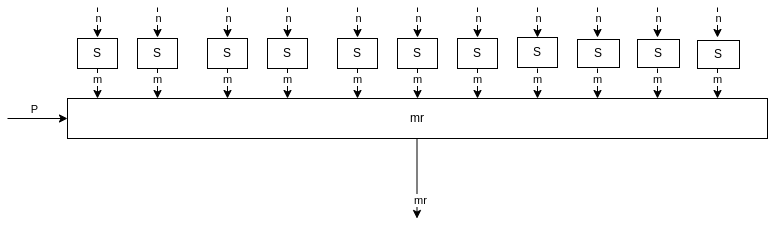
\includegraphics[scale=0.6]{Images/L4/SPN.png}\\

$ S\ :\ \{0,1\}^n\ \rightarrow \ \{0,1\}^m ,\\
p\ :\ \{0,\ .\ .\ .\ m_{r-1}\ \rightarrow \{0,\ .\ .\ .\ m_{r-1} \} $

\section{Feistel Network(FN) :}
FN is based also based on block cipher.Also DES is based on FN.\\

\begin{multicols}{2}
\subsection{Encryption :}
$P\ \rightarrow $ plain text of size 2n-bits.
Out of that let's call first n bits $L_0$ and second half $R_0$.\\
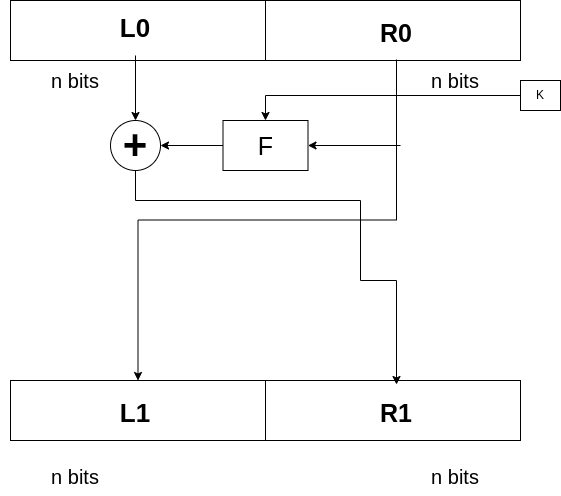
\includegraphics[scale=0.3]{Images/L4/L4_Cryupto_FN.drawio.png}\\
If Cipher text $C=L_1||R_1$.\\
$L_!\ =\ R_0$\\
$R1\ =\ L_1\ \oplus\ f(R_0,k)$

\columnbreak
\subsection{Decryption :}
Plain text \\\\
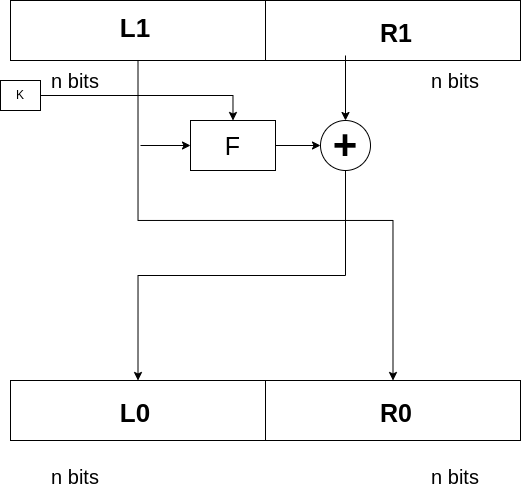
\includegraphics[scale =0.3]{Images/L4/L4_Crypto_FN1.drawio.png}\\\\
$L_0\ =\ R_1\ \oplus\ f(R_0,k)$ $\rightarrow$ $L_0\ =\ R_1\ \oplus\ f(L_1,k)$ \\
$R_0\ =\ L_1$\\
\end{multicols}

\newpage


\section{Iterated block cipher :}
One computation will be iterated for number of rounds.the computation is called round fuunction.\\\\
Parameters of such functions are : \\
number of rounds r,\\
block size n,\\
round key $k_i$ of length l.\footnote{It is generated from the original seceret key k}\\

\subsection{Characteristics of iterative block cipher:}
\begin{enumerate}
    \item no. of rounds n
    \item round function F
    \item Plain text block P
    \item Secret key K
\end{enumerate}

Let's take a 3 round block cipher.
It has 3 rounds and relative keys and we have a key scheduling function \\

$G(n)\ =\ k_1,k_2,k_3$ \\

and those are our round keys.\\
key scheduling functions gives distinct round keys for the secret key as input.


\section{OTP(One time padding):}
OTP provides perfect secrecy under some condition.

\subsection{Encryption :}
$P\ \rightarrow\ $ plain text\\
$K\ \rightarrow\ $ Secret key\\

$Enc(P,k)\ =\ p \oplus k =\ C$

\subsection{decryption :}

$Dec(C,k)\ =\ C \oplus k =\ CP$\\

$P_r[message | Cipher text] = P_r[message]$

%%%%%%%%%%%%%%%%%%%%%%%%%%%%%%%%%%%%%%%%%%%%%%%%%%%%%%%%%%%%%%%%%%%%%
\end{document}
